% !TEX encoding = UTF-8 Unicode

\documentclass[twocolumn,10pt,a4j]{ltjsarticle}
\usepackage{kougai}

\title{アクティブラーニングを用いる講義の雛形の考案}
\author{2032107 土屋 勇太  指導教員 須田 宇宙 准教授}
\date{}

\begin{document}

\maketitle

\section{はじめに}
%1章には,背景・問題点・目的を順番に書く.
%背景は,広く一般的な事柄を書いて,読む人に同意を抱かせつつ問題点につなぐ.
%問題点では,「〜という問題点がある」などのように,「問題」または「問題点」と言う単語を用いて,目的につなぐ.
%目的では,「そこで本研究では」から始めて,「〜を目的とする」で締める.
%以下は過去の卒業研究最終審査用の梗概の抜粋である.

%背景
近年,社会的変化が加速し,先を予測することが困難とされている.
そのため社会全体で,変化に対して受け身でいるのではなく,自ら変化に対して積極的に学び取り入れる姿勢や能力が求められるようになった.
文部科学省は,2020年度に改定された学習指導要領にて「『主体的・対話的で深い学び』の実現に向けた授業改善の推進」を行い,アクティブラーニングを推奨した.
同様に経済産業省は,2017年に新たに「人生100年時代の社会人基礎力」を定義した.
「主体性」や「課題発見力」,「実行力」などの12の項目から構成され,社会人として現代を生きる上で必要な能力を示している.
以上の背景から,様々な教育の場においてグループワークやPBL教育などのアクティブラーニングが用いられるようになった.
中でも,大学は知識を幅広く学び専門的な研究を行うことで,論理的思考力や課題を発見・解決する能力といった応用力を身につける場であるとされている\cite{daigaku}.

%問題点
しかし,現在大学で実施されているアクティブラーニングの多くは,出席率の向上や学習内容の定着を目的に実施しており,「論理的思考力」や「課題発見力・解決力」といった大学の講義やアクティブラーニングの本来の目的や効果が重視されていないという問題がある.

%目的
そこで本研究では,自ら学習する「主体性」や「論理的思考力」,「課題発見力・解決力」を身につけることのできる大学講義の雛型を考案することを目的とする.



\section{アクティブラーニングの問題点}
%その他,数式を用いて理論を説明することも可能である.
図\ref{fig:ピラミッド}に示すラーニングピラミッドと呼ばれる考え方があり,講義や読書よりもグループでの討論や人に教える体験などの方が学習内容の定着率が高いとされている.
また,学習内容の定着率の高い学習を,アクティブラーニングと称して実施する取り組みが存在している.
しかし,本来のアクティブラーニングの目的は「主体性」や「論理的思考力」,「課題発見力・解決力」などの能力を身につけることである.
%しかし,実施されているものでは主体性や論理的思考力,課題発見力・解決力の育成には繋がりにくいという問題がある.
%アクティブラーニングとは,学習者の能動的な参加を取り入れた学習方法の総称であり,主体性や,論理的思考力,課題発見力・解決力を養うことができる.
%アクティブラーニングとは,学習者の能動的な参加を取り入れた学習方法の総称であり,主体性や,論理的思考力,課題発見力・解決力を養うことができる.
%本来,学習は主体的な方法で学習をした方がより内容の定着率が高いという効果がある.
%この効果を示した研究をラーニングピラミッドという.概要を図に示す.
%講義や読書といった受動的な学習だと内容の定着率が低いが,グループでの討論や他者に教えるなどといった自ら主体的に学ぶ方法では定着率が高い.
%また,ラーニングピラミッドにおいてアクティブラーニングは「グループ討論」から「人に教える」に該当する.
%しかし,内容の定着や内容に興味を持たせるきっかけを与えるものとして実施されていることが多く,主体性や論理的思考力,課題発見力・解決力の育成には繋がりにくいという問題がある.
%アクティブラーニングとは,学習者の能動的な参加を取り入れた学習方法の総称である.
%主体性や,論理的思考力,課題発見力・解決力を養うことができる.
%また,アクティブラーニングのような主体的な学習には学習内容の定着率を上げるという効果もある\cite{piramid}.
%この効果を示した研究をラーニングピラミッドという.概要を図\ref{fig:ピラミッド}に示す.
%なお,アクティブラーニングはラーニングピラミッド内の「グループ討論」から「人に教える」に該当する.
%しかし,内容の定着や内容に興味を持たせるきっかけを与えるものとして実施されていることが多く,主体性や論理的思考力,課題発見力・解決力の育成には繋がりにくいという問題がある.

\begin{figure}[b]
\begin{center}
 \includegraphics[clip,width=85mm]{図1.pdf}
\end{center}
 \caption{ラーニングピラミッド}
 \label{fig:ピラミッド}
\end{figure}

%\begin{figure}[h]
%\begin{center}
 %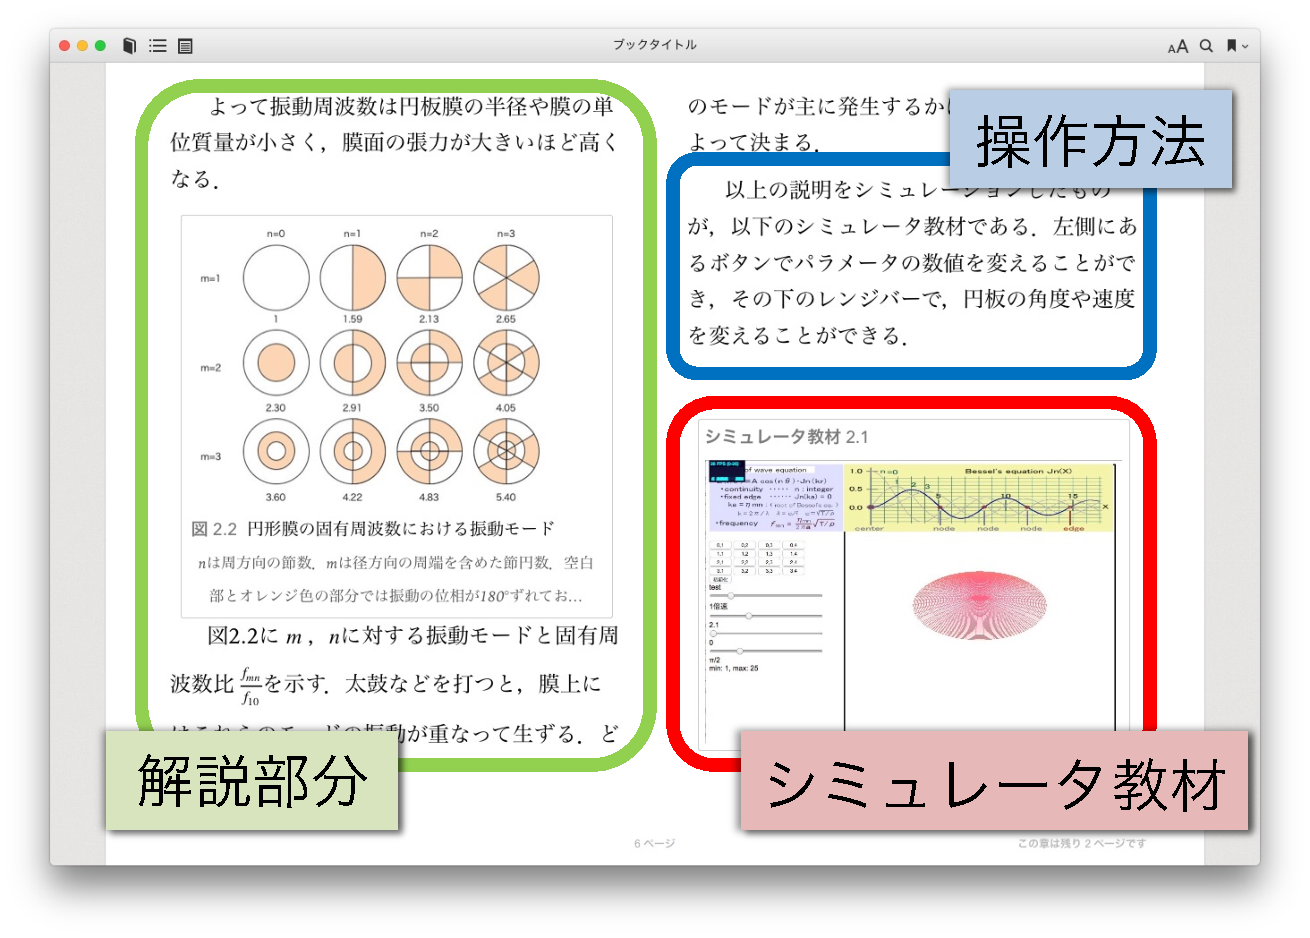
\includegraphics[clip,width=85mm,height=40mm]{textbook.pdf}
%\end{center}
% \caption{電子教科書サンプル}
 %\label{fig:教科書}
%\end{figure}

\section{研究の構想}
本研究で目標とする能力を身につけるためには,それぞれ手法が必要であると考えた.
目標とする能力と身につけるためのそれぞれの手法を表\ref{table:data_type}に示す.
例えば,目標とする「主体性」の能力を身につけるために,「目標の設定・確認」,「グループ活動」,「進行の方法や手順の確認」の手法を実施することが必要であると考えた.
加えて,事前の準備として内容に対する最低限の知識・技術の講義と,自己や外部など様々な角度からの振り返りも必要と考えた.
また,本研究の対象は大学の講義であるため,1時間の講義を3回〜5回行う中で,事前指導から振り返りまでを含む表\ref{table:data_type}の手法を適当に取り入れ組み立てることで,各能力を身につけられる講義を考案する.

\begin{table}[b]
  \caption{能力に応じた必要項目}
  \label{table:data_type}
  \centering
  \begin{tabular}{ll}
  \hline
    目標とする能力   &  能力を身につけるための手法  \\
    \hline \hline
    主体性  & 目標の設定・確認   \\
    		& グループ活動\\
		& 進行の方法や手順の確認\\ \hline
    論理的思考力  & 討論  \\
    			& 調べ学習  \\
			& 発表などのアウトプット \\ \hline
    課題発見力  &  討論\\
    			&  調べ学習\\ \hline
    課題解決力  &  図や表の作成 \\
    			& 発表などのアウトプット \\ \hline \hline
	
	事前準備  &  最低限の知識・技術の講義 \\ \hline
    	振り返り& 自己評価 \\
			& 相互評価 \\
			& 外部評価 \\
    \hline
  \end{tabular}
\end{table}



\section{今後の予定}
%中間審査用の梗概では4章のタイトルとして「今後の予定」,最終審査用の梗概では「おわりに」などを用いる.
%たいてい2〜3行程度でまとめる.

今後は表\ref{table:data_type}の内容を基に手法を組み合わせ,講義の流れを計画する.また,実施方法や時間配分,評価方法についても検討し講義を考案する.


\begin{thebibliography}{99}
\bibitem{daigaku} 文部科学省:``大学の目的'',\url{https://www.mext.go.jp/b_menu/shingi/chukyo/chukyo4/003/gijiroku/attach/1414357.htm}, 2023/7/17参照


\end{thebibliography}

\end{document}
